\documentclass[11pt, a4paper, twocolumn]{article}

% --- Paquetes de Idioma y Codificación ---
\usepackage[utf8]{inputenc}
\usepackage[spanish, es-nodecimaldot]{babel} % Configurado para español
\usepackage[T1]{fontenc}

% --- Tipografía y Estética ---
\usepackage{mathpazo} % Fuente Palatino, elegante y legible
\usepackage{microtype} % Mejora el espaciado entre letras y palabras

% --- Geometría de Página ---
\usepackage[margin=2.5cm, top=3.8cm, headheight=65pt, headsep=0.8cm]{geometry}
\columnsep 0.6cm % Espacio entre columnas

% --- Matemáticas Avanzadas ---
\usepackage{amsmath, amsfonts, amssymb, amsthm}
\usepackage{amsmath}
\usepackage{mathtools}
\usepackage{mathtools}
\usepackage{appendix}
% --- Gráficos y Tablas ---
\usepackage{graphicx}
\usepackage{booktabs} % Para tablas con estilo profesional (sin líneas verticales)
\usepackage{caption}
\usepackage{svg}
\usepackage{dblfloatfix}

\captionsetup{labelfont=bf, font=small} % Captions en negrita y pequeñas

% --- Hipervínculos y Referencias ---
\usepackage[colorlinks=true, allcolors=blue]{hyperref}
\usepackage[capitalize]{cleveref} % Referencias inteligentes (ej: Fig. 1)
\usepackage{biblatex}
\usepackage{csquotes}
\addbibresource{referencias.bib}

% --- Título y Autores ---
\title{\textbf{\Large Experimento de Franck-Hertz}}
\author{
	\textbf{Truchado Iniesta, Eduardo}, \textbf{Sanz Rubio, Juan} \\
	\small Grado de Física, UCLM. \texttt{juan.sanz1@alu.uclm.es} \\
	\small Grado de Física, UCLM. \texttt{eduardo.truchado@alu.uclm.es}
}
\date{\small 2 Marzo 2026}


\usepackage{fancyhdr}
%\usepackage{graphicx}

% --- Configuración del Encabezado ---
\pagestyle{fancy}
\fancyhf{} % Limpia encabezado y pie de página
\renewcommand{\headrulewidth}{0.4pt} % Línea horizontal bajo el encabezado

% Imagen a la IZQUIERDA
\fancyhead[L]{
\includegraphics[height=2cm]{logoFCTo.png}}

\fancyfoot[C]{\thepage}


\fancypagestyle{plain}{
	\fancyhf{} % Limpia el estilo plain por defecto
	\fancyhead[L]{
\includegraphics[height=2cm]{logoFCTo.png}} % Mantiene tu logo
	\fancyfoot[C]{\thepage} % Fuerza el número de página
	\renewcommand{\headrulewidth}{0.4pt} % Mantiene la línea
}

% --- Inicio del Documento ---

\begin{document}

\maketitle
\thispagestyle{fancy}

%Resumen

\begin{abstract}

En esta práctica nuestro objetivo será verificar experimentalmente la 
cuantización de los niveles de energía atómicos. Para ello, realizaremos 
el experimento de Franck-Hertz, en el que aceleraremos electrones mediante 
una diferencia de potencial variable y estudiaremos sus colisiones con átomos 
de mercurio en fase gaseosa. A partir de la curva característica 
corriente-voltaje obtenida, determinaremos experimentalmente la energía del 
primer nivel de excitación del mercurio y la compararemos con el valor 
teórico de $4,9 eV$.

\end{abstract}


\section{Introducción}

Según los postulados de Bohr, los electrones en los átomos solo pueden ocupar 
niveles de energía discretos, o cuantizados, y por lo tanto solo pueden emitir 
y absorber electrones cuya energía corresponda al salto entre dos niveles:

\begin{equation}
   \Delta E = E_f - E_i = h\nu
\end{equation}

Para comprobar la veracidad de este postulado tenemos el experimento de 
Franck y Hertz. Este experimento consiste en bombardear a átomos con electrones con una 
energía cinética conocida:

\begin{equation}
   K = \frac{1}{2}mv^2 = |e|V
\end{equation}

donde $e$ es la carga del electrón y $V$ la tensión aceleradora aplicada. 
Cuando la energía cinética de los electrones es inferior a la energía del 
primer nivel excitado del átomo, las colisiones que se producen son 
elásticas: el electrón no transfiere energía interna al átomo y ambos 
conservan su energía cinética. Por el contrario, cuando la tensión 
aceleradora es suficiente para que el electrón alcance dicha energía umbral, 
la colisión pasa a ser inelástica y el electrón cede exactamente esa energía 
al átomo, excitando a uno de sus electrones a un nivel superior.

\vspace{0.2cm}

En el montaje experimental se utiliza un tubo de Franck-Hertz relleno de 
vapor de mercurio a baja presión, en el que los electrones son emitidos por 
efecto termoiónico desde un cátodo calefactado y acelerados hacia una rejilla 
mediante la tensión $U_1$. Una pequeña tensión de frenado $U_2$ aplicada entre 
la rejilla y el ánodo colector impide que lleguen al detector aquellos 
electrones que hayan perdido su energía en una colisión inelástica:

\begin{figure}[h]
	\centering
	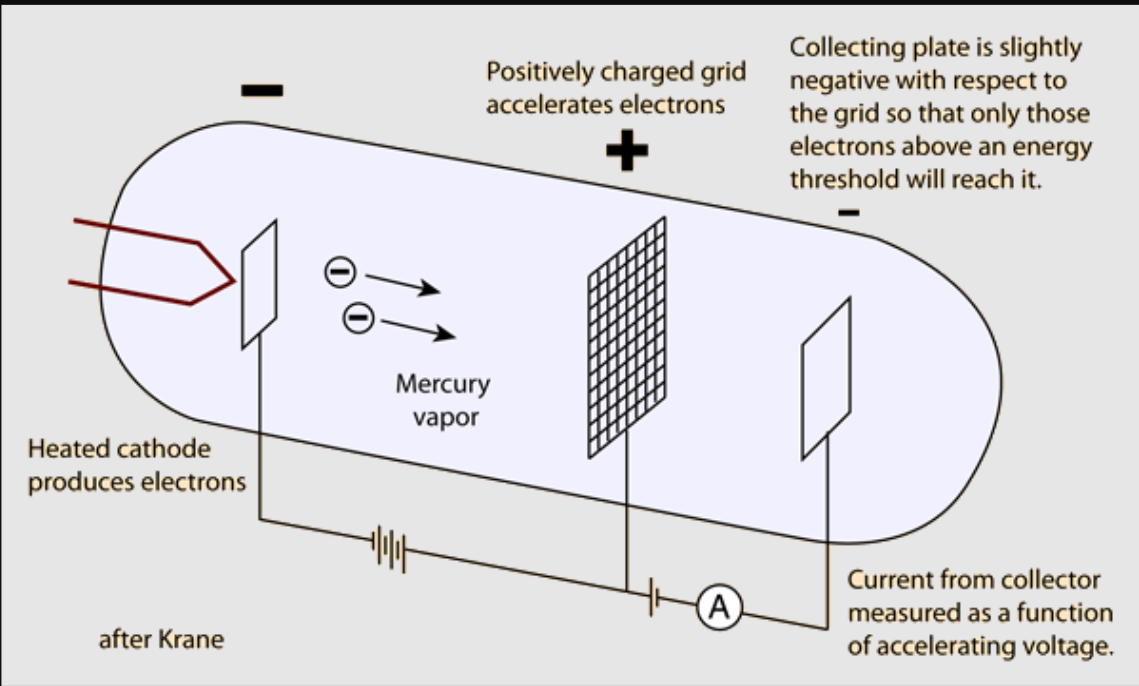
\includegraphics[scale=0.2]{imagenes/TuboFrankHertz.png}
	\caption{Tubo de Frrank-Hertz de \cite{FrankHertzTubo}}
	\label{TuboFrankHertz}
\end{figure}

Al aumentar progresivamente $U_1$, la corriente anódica crece hasta que los 
electrones alcanzan la energía de excitación del mercurio 
momento en el que se produce una caída brusca de la corriente. Al seguir 
aumentando $U_1$, los electrones recuperan energía cinética tras la colisión y 
la corriente vuelve a crecer, repitiéndose el proceso periódicamente. La 
curva $I_A$-$U_1$ resultante presenta así una serie de máximos y mínimos 
equiespaciados, cuya separación en tensión corresponde directamente a la 
energía del primer nivel de excitación del átomo de mercurio, confirmando 
la cuantización de los niveles energéticos predicha por Bohr.




\section{Objetivos}
Los objetivos de esta práctica serán: verificar la cuantización de los niveles 
de energía y calcular el valor experimental de esos niveles de energía.


\section{Metodología}

Conectamos el equipo Franck-Hertz, que tiene un circuito tal que:

\begin{figure}[h]
	\centering
	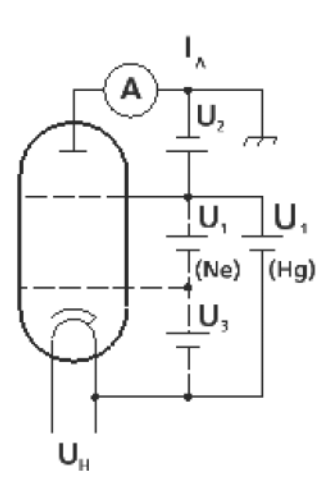
\includegraphics[scale=0.5]{imagenes/CircuitoHertz.png}
	\caption{Circuito del dispositivo Franck-Hertz}
	\label{CircFH}
\end{figure}

donde $U_H$ es la tensión que se aplica al filamento que actua de calentador, $U_1$
es la tensión aceleradora; que se encarga de acelerar los electrones arrancados a 
la resistencia, $U_2$ es la tensión de frenado; que se encarga de frenar a los 
electrones que no vengan con la energía cinética suficiente y $U_3$ es una tensión 
de aceleración extra que al no ser necesaria para el mercurio mantendremos siempre 
como 0.

\vspace{0.2cm}

Con el montaje hecho, prepararemos el horno a una temperatura de $T=175ºC$ y 
esperaremos a que alcance ese valor, luego, esperaremos unos 15 minutos adicionales 
para asegurarnos de que se encuentra a esa temperatura en todo el tubo. Y cada vez 
que variemos la temperatura repetiremos este proceso.

\vspace{0.2cm}

A la hora de medir, tomaremos dos valores, la tensión $U_1$ y la diferencia 
de potencial generada por la corriente anódica $I_A$. Y lo que haremos será 
hacer un barrido en modo "sierra" del voltaje $U_1$ de $1V$ a $60$ mientras 
que mantenemos $U_2$ a una tensión constante a $2V$ y $U_H$ a $6.3 v$.

\vspace{0.2cm}

Además, el dispositivo Franck-Hertz que utilizamos tiene dos salidas para 
medir directamente estas dos variables de interés, tan solo las recogeremos 
con un osciloscopio para poder tomar medidas. En esta práctica utilizaremos 
tres osciloscopios diferentes: un osciloscopio analógico, un primer osciloscopio 
digital (PicoScope 2202) y un segundo osciloscopio digital (Analog Discovery).

\vspace{0.2cm}

Una vez colocadas ambas entradas a cada canal del osciloscopio, seleccionaremos 
el módo de $x-y$ tomando $U_1$ como $x$ y la tensión generada por $I_A$ como $y$ 
ya que solo nos interesa el valor del voltaje de canal, no 
el tiempo. Además, cada uno de ellos tiene una frecuencia de muestreo diferente por lo que 
los resultados, aunque generalmente sean los mismos, tendrán variaciones 
en cuanto a la precisión. 

\section{Tratamiento de datos}

A continuación mostraremos los datos obtenidos al realizar las medidas con
cada osciloscopio. Además, para cada osciloscopio realizaremos 3 medidas 
diferentes a diferentes temperaturas: $T=175K$, $T=170K$ y $T=180K$.


\subsection{Osciloscopio analógico}

Para este osciloscopio no teníamos la opción de obtener los datos directamente 
al ordenador, por lo que tan solo tomamos imagenes del resultado:

\begin{figure}[h]
	\centering
	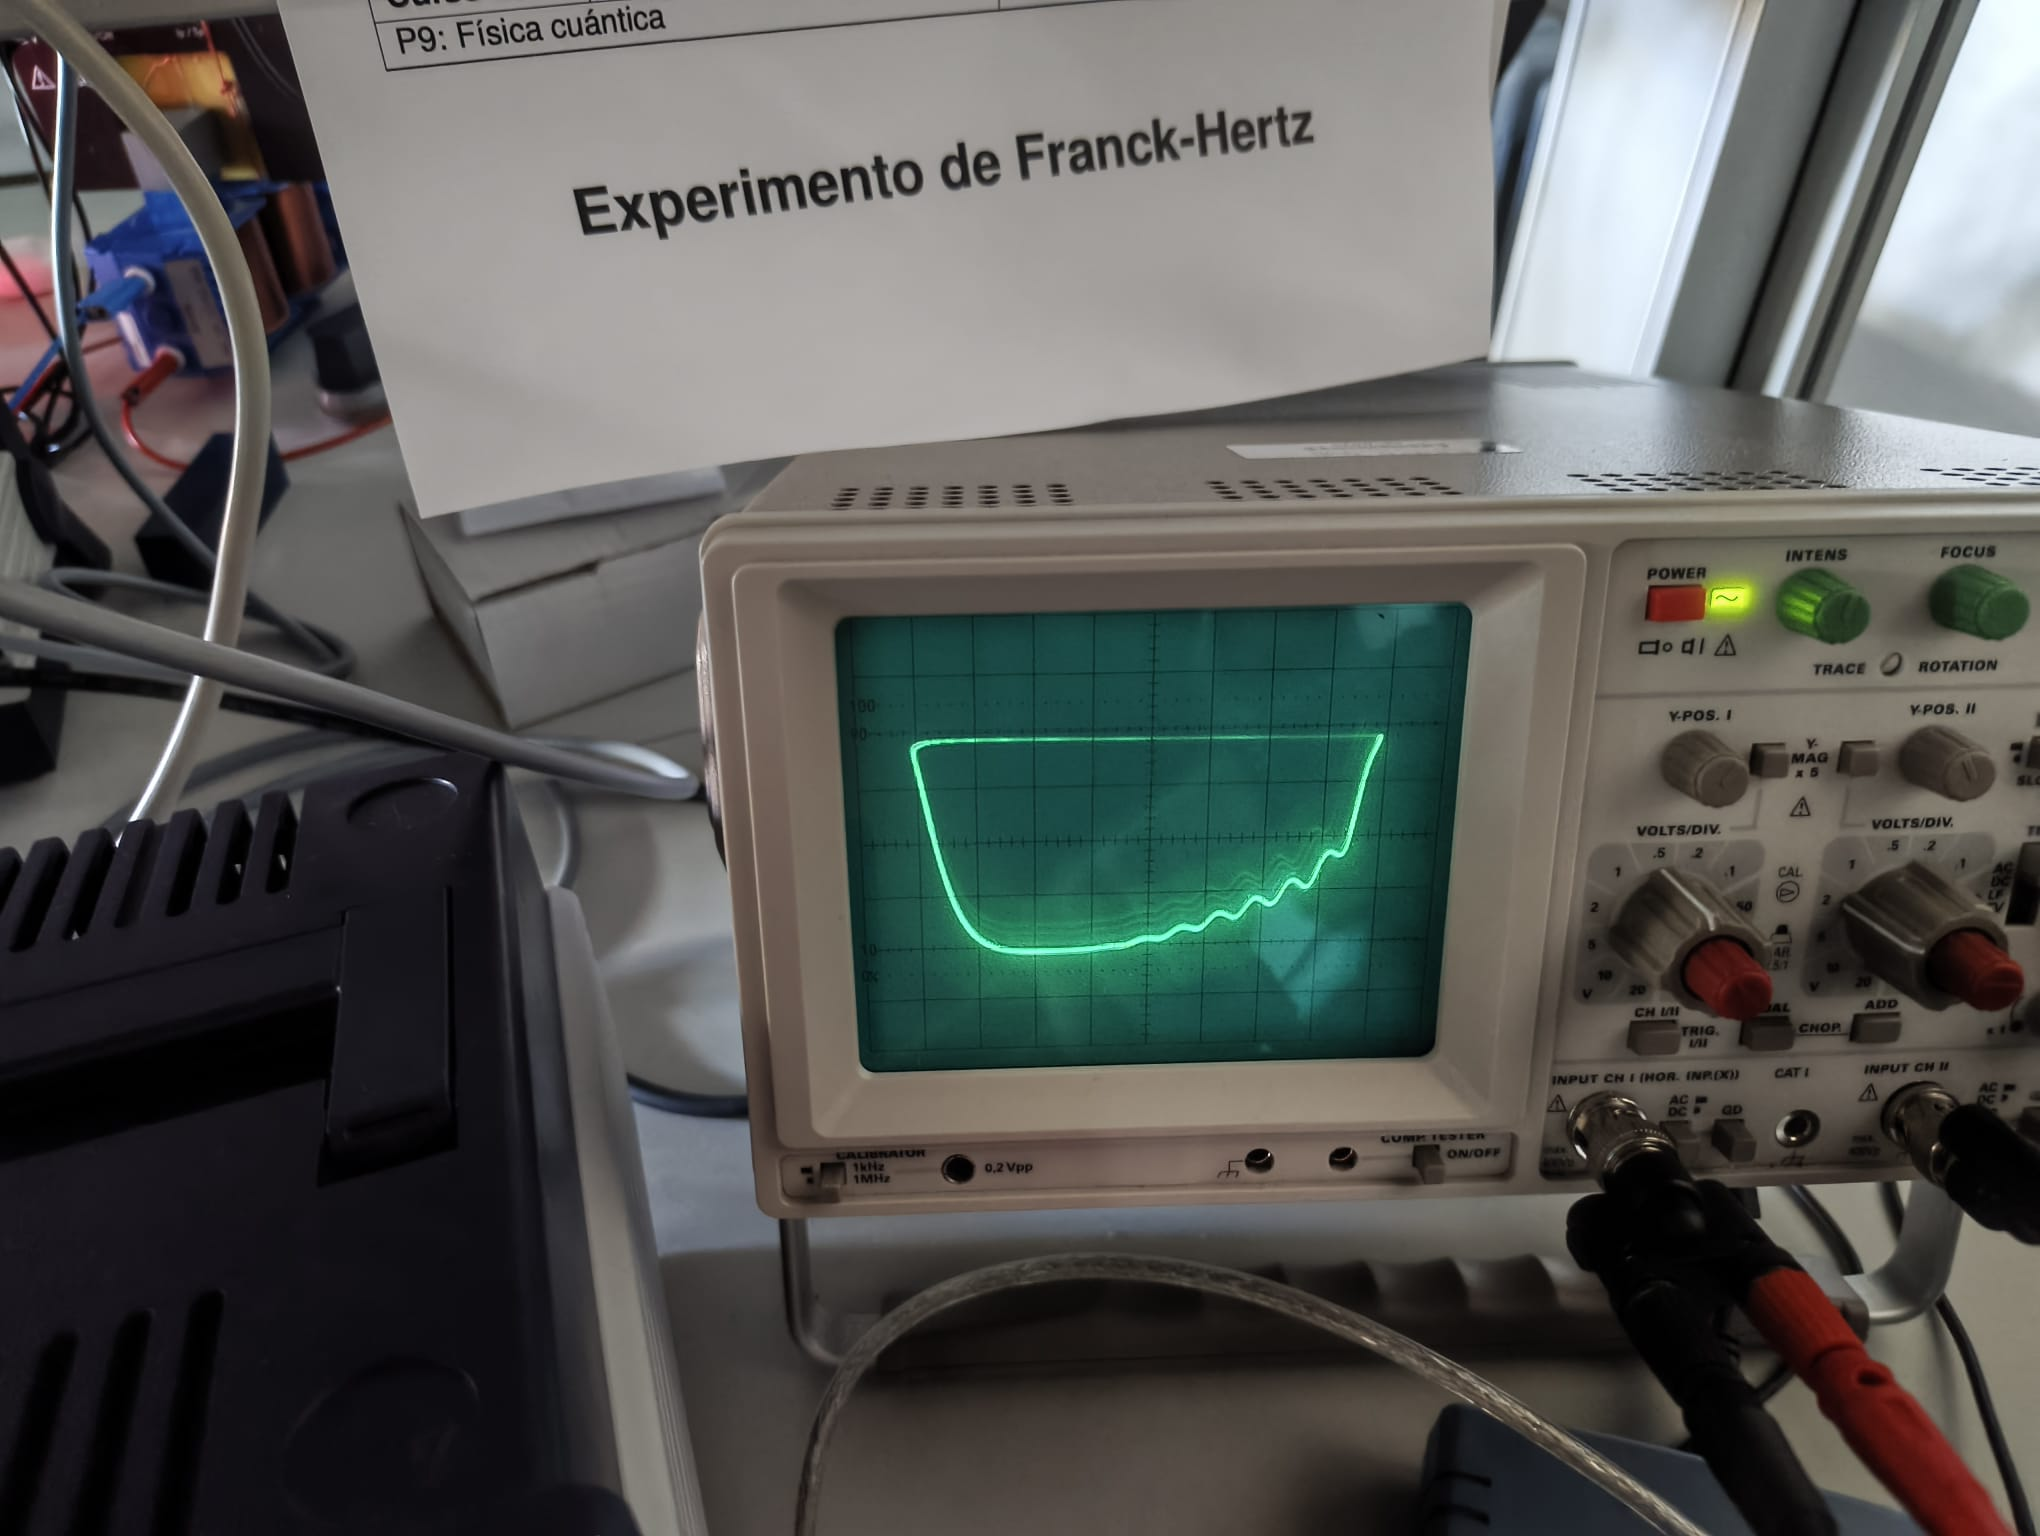
\includegraphics[scale=0.11]{imagenes/T_170_anag.jpg}
	\caption{Resultado del osciloscopio analógico para $T=170^\circ$}
	\label{Anag170}
\end{figure}

\begin{figure}[h]
	\centering
	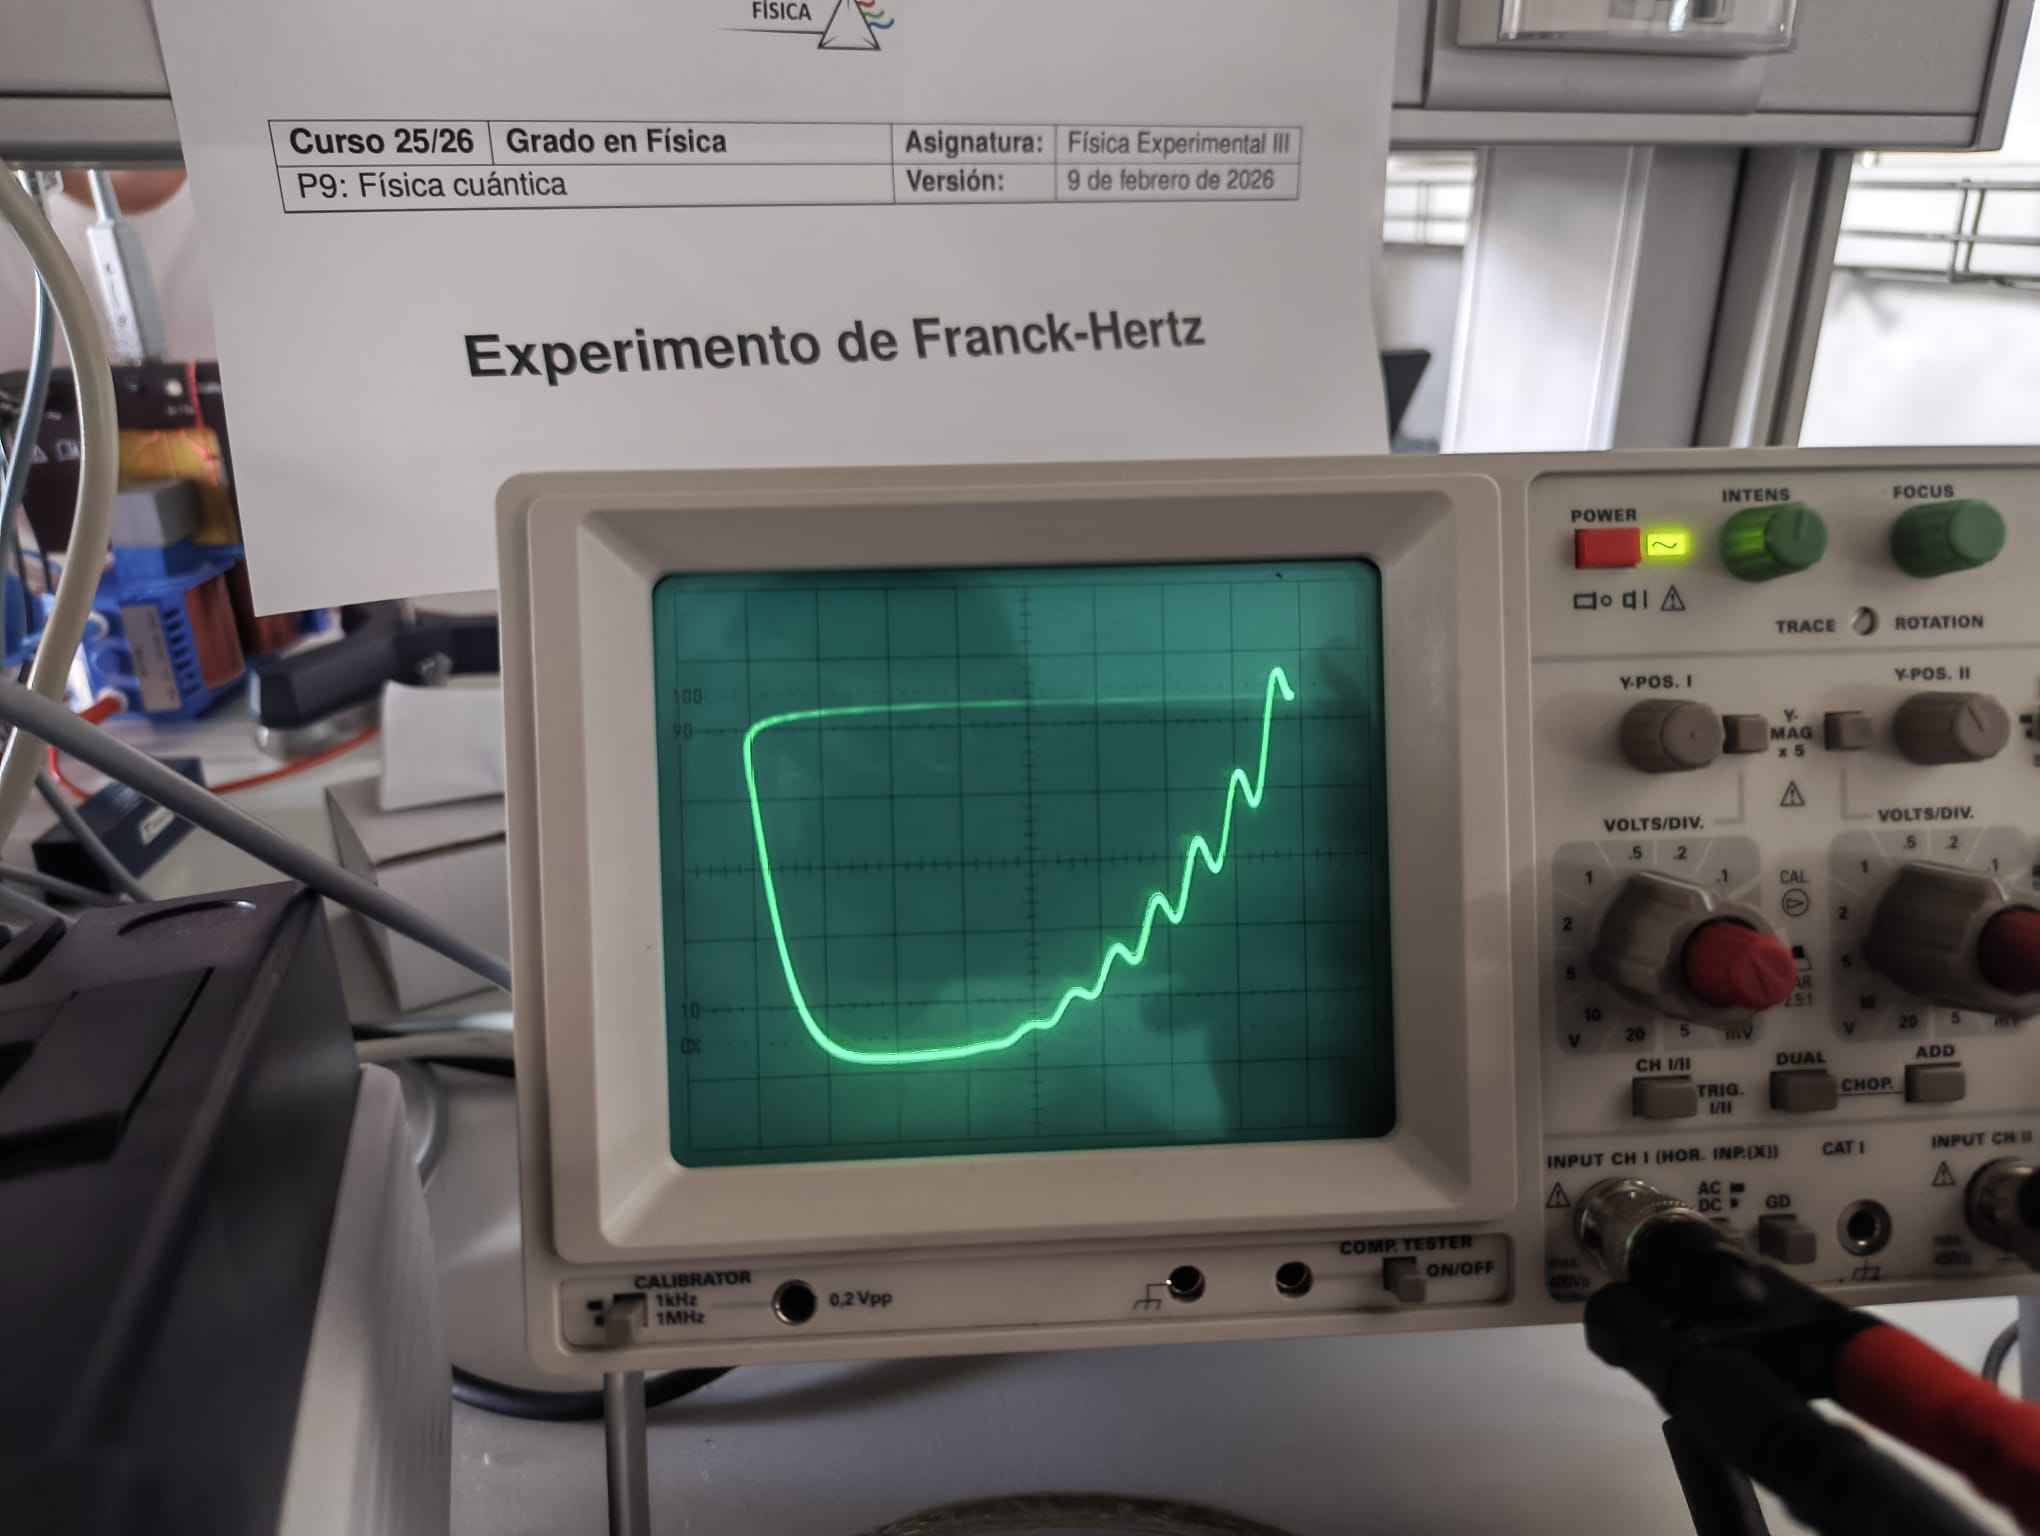
\includegraphics[scale=0.11]{imagenes/T_175_anag.jpg}
	\caption{Resultado del osciloscopio analógico para $T=175^\circ$}
	\label{Anag175}
\end{figure}

\newpage 
\begin{figure}[h]
	\centering
	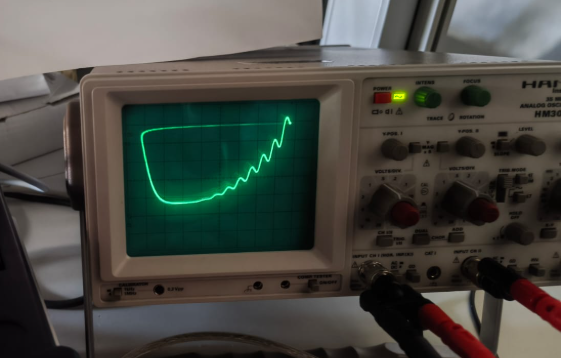
\includegraphics[scale=0.4]{imagenes/T_180_anag.png}
	\caption{Resultado del osciloscopio analógico para $T=180^\circ$}
	\label{Anag180}
\end{figure}

\subsection{PicoScope 2202}

Este osciloscopio ya permite, además de la representación de la gráfica $x-y$, 
la adquisición de datos por ordenador. Sacando un archivo $.csv$ para cada medida.
Lo que haremos será, para cada temperatura obtener 64 mediciones, que correspondrán 
a 64 archivos $.csv$. La representación gráfica que devuelve el software del
osciloscopio es:

\begin{figure}[h]
	\centering
	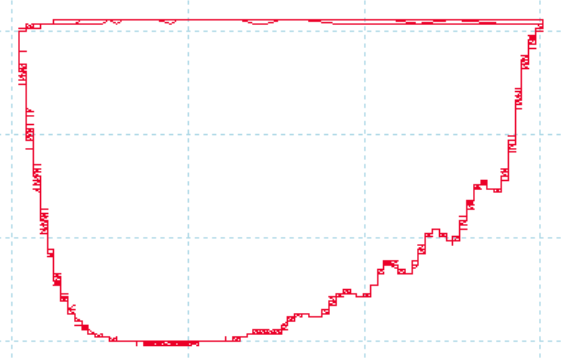
\includegraphics[scale=0.2]{imagenes/T170.png}
	\caption{Resultado del osciloscopio PicoScope 2202 para $T=170^\circ$}
	\label{Pico170}
\end{figure}

\begin{figure}[h]
	\centering
	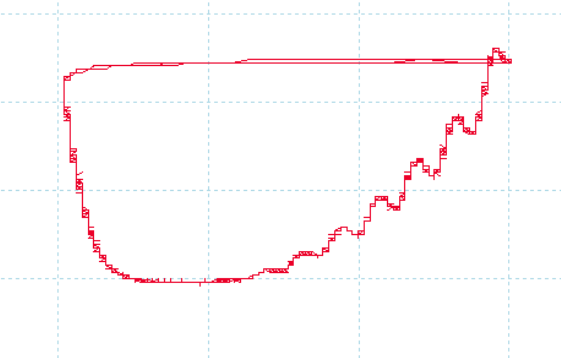
\includegraphics[scale=0.2]{imagenes/T175.png}
	\caption{Resultado del osciloscopio PicoScope 2202 para $T=175^\circ$}
	\label{Pico175}
\end{figure}

\begin{figure}[h]
	\centering
	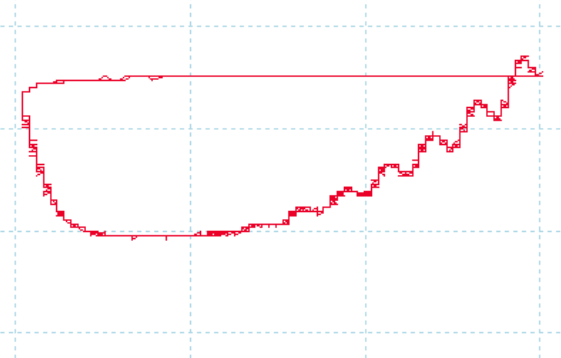
\includegraphics[scale=0.2]{imagenes/T180.png}
	\caption{Resultado del osciloscopio PicoScope 2202 para $T=180^\circ$}
	\label{Pico180}
\end{figure}

Los ficheros de datos se encuentran en \cite{experimental32026} dentro de 
la carpeta correspondiente a esta practica en la ruta "$/Franck\_Hertz/Practica/PicoScope\_2202$".

\subsection{Analog discovery}

Por último, utilizaremos el osciloscopio Analog discovery, que nos devuelve 
los datos en formato $.csv$. La ruta a estos archivos dentro del repositorio de 
github es: "$/Franck\_Hertz/Practica/Analog\_discovery$".

\section{Análisis de resultados}

En esta sección, crearemos un programa en python que calcule la distancia entre los 
mínimos leyendo el archivo de datos.

\section{Conclusiones}

Tras el estudio podemos concluir que la medición de las lineas espectrales 
del mercurio para calibrar la constante de red, pese a no estar dentro de los 
límites de error. Dió un resultado aceptable.

\vspace{0.2cm}

En cuanto a la parte del cálculo de las lineas espectrales, pese a que hemos intentado 
varios métodos como la medida directa y el uso de un fotodiodo, ambas tienen 
mucho error y no se acercan todo lo que deberían al valor esperado. Probablemente 
la fuente de error sea que la medida directa no haya sido todo lo precisa posible 
especialmente a la hora de mantener perpendiculares la muestra y la red de difracción, 
y que en la medida con el fotodiodo este tomaba un ancho de luz demasiado grande 
y cuando enfocabamos a un solo ángulo este tomaba la intensidad de un rango de unos $10º$ 
que supone un tercio de todo el barrido. Esta última parte intentamos compensarla 
añadiendo un tubo mas largo al óptico del goniómetro o tapando con cinta la mayor 
parte del telescopio, pero no resultó en nada.

\vspace{0.2cm}

La mejor manera de resolverlo habría sido, conseguir un tubo mas delgado y que 
filtrase mejor la luz haciendola mas directa y utilizar una red de difracción 
que hubiese dispersado mas las lineas espectrales.

\vspace{0.2cm}

Por otro lado, el uso de la GUI desarrollada y de la literatura nos han hecho 
ver que pese a los errores en el procedimiento no estamos tan alejados de los 
autenticos resultados.

\vspace{1cm}
Para ver todo el análisis de datos realizado por los alumnos, se habilita este 
enlace al repositorio de 
github donde están todos los archivos de prácticas: 
\cite{experimental32026}


\section{Referencias}

\nocite{experimental32026}

%\nocite{cambou2011three}
%\nocite{garcia2012bolas}

\printbibliography

\appendix
\onecolumn




\end{document}